\section{PCA for Model Order Reduction and Bound Computation}

%Some words on PCA, learn of 2 Matrix full-dim to reduced-dim and back.
%Then, how we use it (pictures and text).

Figure~\ref{fig.MNIST} depicts the pipeline used for computing global bounds on the MNIST dataset. Firstly, the MNIST dataset is used to train an MNIST DNN, obtaining 97\% of classification accuracy, as denoted in ``Training''. 
%
In parallel, principal component analysis (PCA) is used to obtain a lower-dimensional representation of the input images, yielding the PCA encoding and the PCA decoding. The PCA encoding transforms the input space (784-dimensional) into a 20-dimensional output image, and the PCA decoding reverses that operation, reconstructing a 784-dimensional image. 
%
The number of retained PCA components is selected to ensure that the MNIST DNN's classification accuracy on reconstructed images (i.e., after PCA encoding and decoding) remains the same as the MNIST DNN used directly on the full-dimensional MNIST images. This phase is referred to as ``Exploitation''. 
%
Lastly, in the ``Bound Computation'' step, we compute an $L_1$ perturbation bound $\varepsilon$. Note that the bound itself is calculated on the full space, even though the bound computation is performed on the 20-dimensional latent space. This is possible since PCA is a \emph{linear operation} based on the eigenvectors of the covariance matrix and its transpose for the PCA decoding (inverse).


%
%It was also used to obtain the PCA encoding and decoding, transforming the images into a reduced basis. The number of PCA dimensions was chosen such that the exploitation accuracy remains constant. That is, encoding into a PCA basis and decoding it results in the same accuracy, as illustrated in ``Exploitation''. 
%
%Last, for the ``bound computation'', we determine an $L_1$-perturbation $\varepsilon$. The search space for bound computation is 20-dimensional. However, the bound itself is computed on the full space. This is possible since PCA is a \emph{linear operation} based on the eigenvectors of the covariance matrix and its transpose for the PCA decoding (inverse).

\begin{figure*}
    \centering
    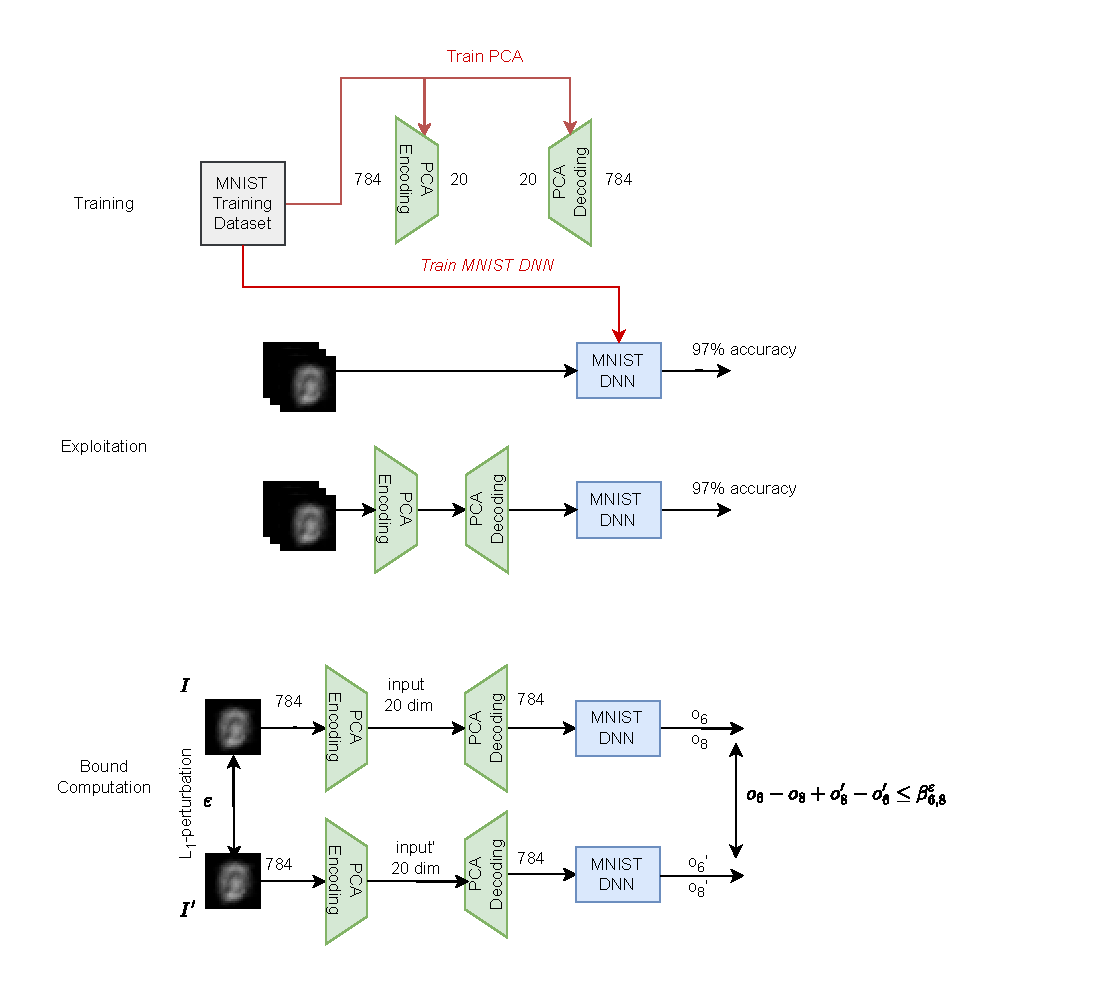
\includegraphics[scale=0.9]{MNIST.pdf} \hspace{1.5cm}
    \caption{Training, exploitation, and bound computation on the MNIST dataset. Note that PCA encoding/decoding used back-to-back can maintain the same accuracy as the original network where PCA is not used. In addition, the bound is computed on the full space even though the analysis is performed on the reduced space. dim = dimension.}
    \label{fig.MNIST}
\end{figure*}	

Figure~\ref{fig.PIPE} illustrates the same pipeline used in the pipe strain case. In this case, two different PCAs are used. The first one is learned with the deformation training dataset, and the second is learned with the plastic strain one.
%
The surrogate is then learned from the reduced deformation to the reduced plastic strain. 
%
For exploitation, we obtain the deformation, use the PCA basis to obtain a reduced deformation, feed the reduced deformation to the surrogate, obtain the reduced strain, and decode the strain (apply PCA inverse), obtaining the strain in the full pipe geometry. Similarly to the MNIST case, we obtain a bound $\varepsilon$ on the input space by solving the MILP problem as proposed on the input dimension.

\begin{figure*}
    \centering
    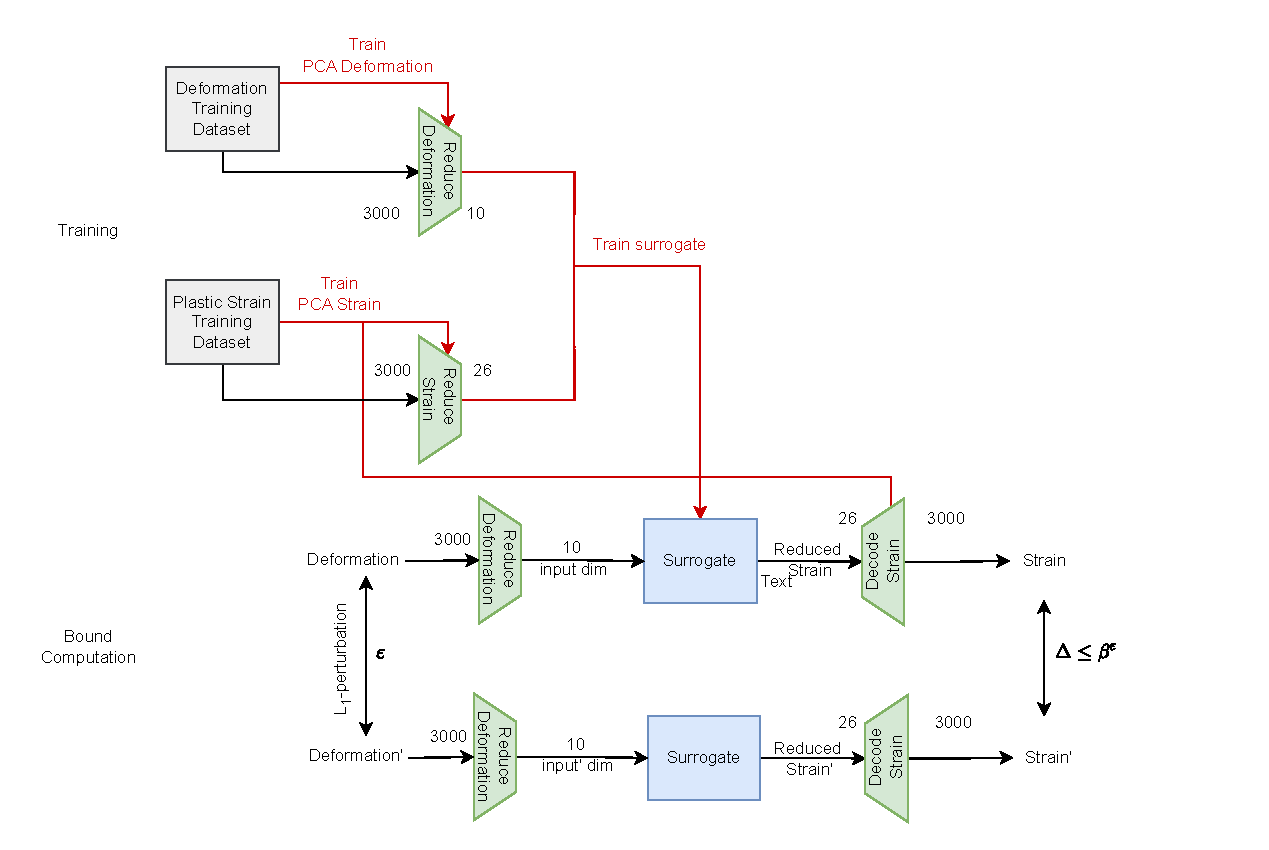
\includegraphics[scale=0.9]{PIPE.pdf} \hspace{1.5cm}
    \caption{Training and bound computation on the pipe use case. Note that two PCAs are used, one for the input space (deformation) and another for the output space (plastic strain). The exploitation and bound computation must then use a pipeline that: (1) reduces the deformation; (2) obtains a reduced strain with the surrogate, and (3) decodes the reduced strain using the PCA inverse. dim = dimension.}
    \label{fig.PIPE}
\end{figure*}	
